\documentclass[spanish]{assignment}

\usepackage{amsmath}
\usepackage{float}

% Title page
\title{Neurocomputación}
\subtitle{Práctica 3 - Autoencoders y series temporales}
\author{Enrique Cabrerizo Fernández\\ Guillermo Ruiz Álvarez}
\date{\today}
\university{Universidad Autónoma de Madrid}

\begin{document}
	\makepre
	\section{Autoencoders.}
	En esta sección se muestran varios resultados obtenidos por el autoencoder para el reconocimiento de caracteres. 
	
	En primer lugar, se ha modificado el fichero \texttt{alfabeto.dat} obteniendo un fichero \texttt{alfabeto.txt} en el que en cada línea se encuentran los 35 atributos representando el caracter correspondiente ($7\times 5$ píxeles por caracter), y 35 datos de salida que son iguales a los de entrada. Este fichero ha sido formateado de tal forma que sea legible por la red neuronal que utiliza \textit{backpropagation} implementado en la práctica anterior, de tal modo que las predicciones son píxeles negros (1) o blancos (0) en función de si cada salida de la red neuronal es mayor, o menor o igual que cero, respectivamente.
	
	La red de retropropagación se ha modificado de tal forma que acepta dos parámetros nuevos:
	\begin{itemize}
		\item \texttt{f\_training:} Indica el número de distorsiones que se añadirán al conjunto de training. 
		\item \texttt{f\_test:} Indica el número de distorsiones que se añadirán al conjunto de test.
	\end{itemize}
	
	En ambos casos, en caso de que el valor del nuevo parámetro sea $n>0$, se generarán 10 versiones ruidosas para cada letra, esto es, se tendrán 10 copias de cada muestra y para cada una de ellas se alerarán $n$ valores aleatorios. En caso de que $n=0$, entonces se omitirá este parámetro, es decir, se realizarán los cálculos sin añadir versiones ruidosas.
	
	El cambio se realizará de la siguiente forma: si $p$ es el valor del píxel a cambiar, el nuevo valor será el siguiente ($\%$ representa la operación módulo, de tal modo que se cambiará el valor $0$ por $1$ y viceversa): $$p = (p + 1) \% 2$$ 
	
	El programa informará, tras la ejecución cual ha sido el valor de \texttt{PE\_Test:} el error promedio cometido en la fase de test medido en \textbf{PE} (píxeles errados por letra).
	
	Tras la modificación del fichero para que la red que utiliza retropropagación pueda tomarlo como entrada, se han realizado tres casos de prueba:
	\begin{itemize}
		\item \textbf{Caso 1:} Tanto el conjunto de entrenamiento como el conjunto de test no contienen versiones ruidosas.
		\item \textbf{Caso 2:} El conjunto de entrenamiento no contiene versiones ruidosas y el conjunto de test contiene 10 versiones ruidosas por cada letra. Se utilizan valores para \texttt{f\_test} de $1, 3$ y $5$.
		\item \textbf{Caso 3:} Tanto el conjunto de entrenamiento como el de test tendrán 10 versiones ruidosas por cada letra. Se utilizan valores para \texttt{f\_training} y \texttt{f\_test} de $1, 3$ y $5$.
	\end{itemize}
	
	\subsection{Caso 1: Abecedario sin ruido.}
	Para este caso se han realizado varias pruebas con distinto número de nodos de la capa interna de la red. El resto de parámetros utilizados son:
	\begin{itemize}
		\item Número máximo de épocas: $200$
		\item Porcentaje de datos utilizado para la fase de training: $100\%$
		\item Porcentaje de datos utilizado para la fase de test: $100\%$
		\item Tasa de aprendizaje: $\alpha = 0.01$
		\item Ruido en fase de training: \texttt{f\_training} $= 0$
		\item Ruido en fase de test: \texttt{f\_test} $= 0$
	\end{itemize}
	
	Los resultados obtenidos son los siguientes:
	\begin{center}
	\begin{tabular}{|c|c|}
		\hline
		\textbf{N.Nodos capa oculta} & \textbf{PE\_Test} \\ 
		\hline
		$10$ & $0.2692$ \\
		$15$ & $0.1154$ \\
		$18$ & $0.0385$ \\
		$20$ & $0.00$ \\
		$25$ & $0.00$ \\
		$30$ & $0.00$ \\
		$35$ & $0.00$\\
		\hline
	\end{tabular}
	\end{center}
	
	Es decir, se tiene que se puede aprender el abecedario completo poniendo un número de neuronas de la capa oculta $\ge 20$. Por lo que no es necesario escoger un subconjunto menor del conjunto total, ya que la red es capaz de aprender el abecedario completo.
	
	\subsection{Caso 2: Conjunto de test con ruido.}
	Para este caso se han realizado diversas pruebas variando el valor del parámetro \texttt{f\_test}, tomando éste los valores $1$, $3$ y $5$. Es decir, se generarán 10 copias ruidosas de cada letra y en cada copia se invertirán $1$, $3$ y $5$ píxeles, respectivamente, en posiciones aleatorias.
	Los parámetros utilizados para las pruebas han sido los siguientes:
	\begin{itemize}
		\item Número máximo de épocas: $200$
		\item Número de nodos en la capa oculta: $25$.
		\item Porcentaje de datos utilizado para la fase de training: $100\%$
		\item Porcentaje de datos utilizado para la fase de test: $100\%$
		\item Tasa de aprendizaje: $\alpha = 0.01$
		\item Ruido en fase de training: \texttt{f\_training} $= 0$
	\end{itemize}

	Los resultados obtenidos son los siguientes:
	\begin{center}
		\begin{tabular}{|c|c|c|}
			\hline
			\textbf{f\_test} & \textbf{PE\_Training} & \textbf{PE\_Test} \\ 
			\hline
			$1$ & $0.00$ & $0.1192$ \\
			$1$ & $0.00$ & $0.1577$ \\
			$1$ & $0.00$ & $0.1423$ \\
			\hline
			$3$ & $0.00$ & $0.8769$ \\
			$3$ & $0.00$ & $0.8154$ \\
			$3$ & $0.00$ & $0.8038$ \\
			\hline
			$5$ & $0.00$ & $2.1231$ \\
			$5$ & $0.00$ & $2.0923$ \\
			$5$ & $0.00$ & $2.1269$ \\
			\hline
		\end{tabular}
	\end{center}
	
	Como se puede observar, en todo momento la red aprende sin fallos todo el abecedario (el valor de \texttt{PE\_training} es siempre $0$), ya que no se alteran los datos en la fase de training y se ha elegido utilizar $25$ neuronas en la capa oculta. Sin embargo, el número medio de errores cometidos en la fase de test es distinto de cero en todos los casos debido al ruido introducido. 
	
	Aún así, incluso con el ruido introducido, el número de errores promedio que se ha cometido en la fase de test (\texttt{PE\_Test}) es siempre menor que el número de alteraciones introducidas (\texttt{f\_test}). Por lo que la red neuronal es capaz de disminuir el ruido introducido.
	
	\subsection{Caso 3: Conjuntos de training y test con ruido}
	Para este caso se han realizado diversas pruebas variando tanto el valor del parámetro \texttt{f\_training} como el valor del parámetro \texttt{f\_test}, tomando estos los valores $1$, $3$ y $5$. Es decir, para ambos conjuntos de training y test se generarán 10 copias ruidosas de cada letra y en cada copia se invertirán $1$, $3$ y $5$ píxeles, respectivamente, en posiciones aleatorias.
	Los parámetros utilizados para las pruebas han sido los siguientes:
	\begin{itemize}
		\item Número máximo de épocas: $200$
		\item Número de nodos en la capa oculta: $25$.
		\item Porcentaje de datos utilizado para la fase de training: $100\%$
		\item Porcentaje de datos utilizado para la fase de test: $100\%$
		\item Tasa de aprendizaje: $\alpha = 0.01$
	\end{itemize}
	
	\newpage
	Los resultados obtenidos son los siguientes:
	\begin{center}
		\begin{tabular}{|c|c|c|c|}
		\hline
		\textbf{f\_training} & \textbf{f\_test} & \textbf{PE\_Training} & \textbf{PE\_Test} \\ 
		\hline
		$1$ & $1$ & $0.0000$ & $0.0538$\\
		$1$ & $1$ & $0.0000$ & $0.0615$\\
		$1$ & $1$ & $0.0115$ & $0.0692$\\
		\hline
		$3$ & $3$ & $0.0038$ & $0.5346$\\
		$3$ & $3$ & $0.0000$ & $0.4077$\\
		$3$ & $3$ & $0.0038$ & $0.4269$\\
		\hline
		$5$ & $5$ & $0.0038$ & $1.4654$\\
		$5$ & $5$ & $0.0154$ & $1.4923$\\
		$5$ & $5$ & $0.0692$ & $1.3962$\\
		\hline
		\end{tabular}
	\end{center}
	
	Se puede observar que esta vez sí que varía el valor de \texttt{PE\_Training} debido al ruido introducido en el entrenamiento. Sin embargo, el error promedio cometido durante la fase de entrenamiento no llega a $0.1$ píxeles por letra. Esto implica que a veces la red no es capaz de aprender al $100\%$ el abecedario completo, sin embargo, al ser entrenada con varias muestras con ruido introducido y siempre la salida correcta, es capaz de disminuir de manera importante el ruido introducido en la fase de test.
	
	En la siguiente tabla se muestra una comparación de los valores de \texttt{PE\_Test} entre el \textbf{Caso 2} y el \textbf{Caso 3}.
	
	\vspace{5mm}
	\noindent\makebox[\textwidth][c]{
		\begin{tabular}{|c|c|c|}
			\hline
			\textbf{Caso 2: PE\_Test} & \textbf{Caso 3: PE\_Test} & \textbf{\% de mejora}\\ 
			\hline
			$0.1192$ & $0.0538$ & $121.56\%$ \\
			$0.1577$ & $0.0615$ & $156.42\%$ \\
			$0.1423$ & $0.0692$ & $105.64\%$ \\
			\hline
			$0.8769$ & $0.5346$ & $64.03\%$ \\
			$0.8154$ & $0.4077$ & $100.00\%$ \\
			$0.8038$ & $0.4269$ & $88.29\%$ \\
			\hline
			$2.1231$ & $1.4654$ & $44.88\%$ \\
			$2.0923$ & $1.4923$ & $40.21\%$ \\
			$2.1269$ & $1.3962$ & $52.34\%$ \\
			\hline
		\end{tabular}
	}
	\vspace{5mm}
	
	En la tabla se muestra el porcentaje de mejora del error obtenido en el \textbf{caso 2} y el \textbf{caso 3}. Se puede observar que en todo momento se supera el $40\%$ de mejora. Por tanto, aunque haya casos en los que la red no pueda aprender el abecedario completo con ruido introducido, se obtienen mejores resultados a la hora de predecir datos con ruido.
		
	\newpage
	\section{Series temporales.}
	\subsection{Código Implementado.}
	La implementación para los primeros cuatro ejercicios de series temporales se encuentran en la carpeta \textbf{bp/} (scripts) y en la subcarpeta \textbf{bp/src} (funciones).\\

	Para adaptar el fichero se ha creado el script \textit{adapta\_fichero.m} que hace uso de la función \textit{adapta\_fichero\_serie} implementada acorde a las especificaciones del ejercicio 1.\\
	
	Para cumplir lo pedido en los ejercicios 2 y 3, se han creado copias de las funciones de entrenamiento de perceptron lineal \textit{bp\_train.m} y \textit{network\_test.m} y se han adaptado al nuevo código cambiando las funciones de transferencia y computando el error cuadrático medio en test. Dichas funciones se encuentran en \textit{bp\_train\_time.m} y \textit{network\_test\_time.m}. Los scripts que ejecutan los ejercicios de series temporales son \textit{series.m} y \textit{series\_recursive.m}, este último, como pide el ejercicio 8, se apoya en la función \textit{predice\_recursivamente.m}.
	
	\subsection{Ejercicio 5.}
	En la siguiente figura podemos ver la gráfica correspondiente a la serie temporal \textit{p3\_serie1.txt}.
	
		\begin{figure}[H]
			\centering
			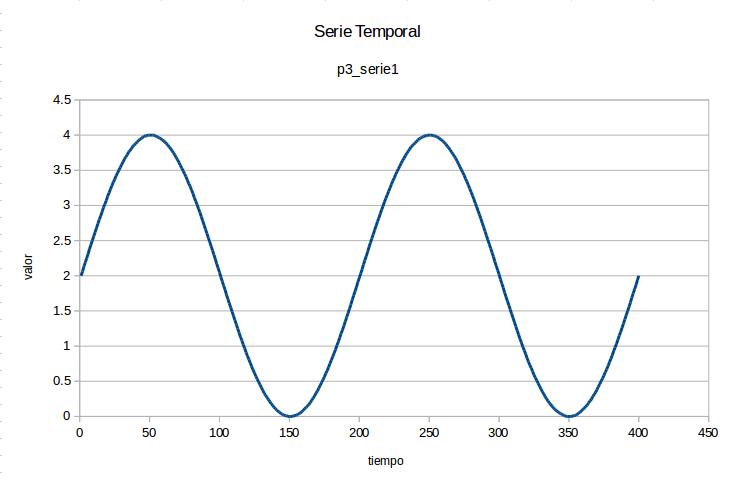
\includegraphics[scale=0.4]{p3_serie1.png}		
			\caption{Serie temporal del fichero \textit{p3\_serie1.txt}.}				
		\end{figure}
	
	Como se puede comprobar es una serie temporal bastante sencilla (es periódica) que se corresponde con una ecuación sinusoidal. La expresión explícita de la serie que representa es:
	
	\begin{align*}
		valor(t) = 2 + 2sin\left(\frac{\pi}{100}t\right)
	\end{align*}
	
	\subsection{Ejercicios 6 y 7.}
	A continuación se muestra una tabla con los valores del error cuadrático medio obtenido para las predicciones y la predicción básica con las diferentes pruebas realizadas.
	
	\vspace{5mm}
	\noindent\makebox[\textwidth][c]{
		\begin{tabular}{|c|c|c|c|c|c|c|}
			\hline
			& \multicolumn{2}{c|}{\textbf{NA=1}} & \multicolumn{2}{c|}{\textbf{NA=2}} & \multicolumn{2}{c|}{\textbf{NA=5}} \\ \hline
			Training \%&     25\%      &     50\%      &      25\%     &      50\%     &      25\%     &      50\%     \\ \hline
			MSE &     0.613495      &     0.183084      &     0.403417      &     0.035622      &     0.087812      &      0.038827     \\ \hline
			MSE básico &      0.002003     &      0.002002     &     0.001993     &      0.002002     &     0.1982     &      0.001985     \\ \hline
		\end{tabular}
	}
	\vspace{5mm}
	
	Como se puede comprobar, los errores son mayores con la predicción realizada con el perceptrón que con la predicción básica, lo que nos indica que en general no está resultando un buen método para resolver el problema. Podemos ver sin embargo que los mejores valores de error se encuentran para $Na = 2$.\\
	
	Indagando en este aspecto, podemos ver que el seno es una función que cumple $sin''(t) = -sin(t)$. La segunda derivada la podemos aproximar como combinación lineal de los valores en $sin(t)$,$sin(t-1)$ y $sin(t-2)$, de forma que la función seno en $t$ se puede aproximar linealmente con los valores en $t-1$ y $t-2$.
	No obstante, nuestra función de transferencia (sigmoide bipolar), no es lineal, con lo que la red se ve obligada a trabajar con pesos en una zona en la que la sigmoide sea lo más lineal posible (pesos muy cercanos a 0). Aún así el resultado no es demasiado satisfactorio. Para contrastar este hecho intuitivo, se ha probado a cambiar la función de transferencia a la identidad, logrando un error cuadrático medio en test de $0.000026$ para $Na=2$, mejorando considerablemente el error de la predicción básica.\\
	
	Por otro lado, se puede comprobar que los errores son mayores también cuando entrenamos únicamente con el 25\% del conjunto ya que no enseñamos al perceptrón una oscilación completa de la función seno y por lo tanto no es capaz de aprender a predecir correctamente con valores negativos.\\
	
	En las figuras \ref{pred_no_lineal_ini}-\ref{pred_no_lineal_end} se pueden ver gráficas con las predicciones para los distintos valores de Na y porcentajes de entrenamiento.\\
	
	\begin{figure}[H]
		\centering
		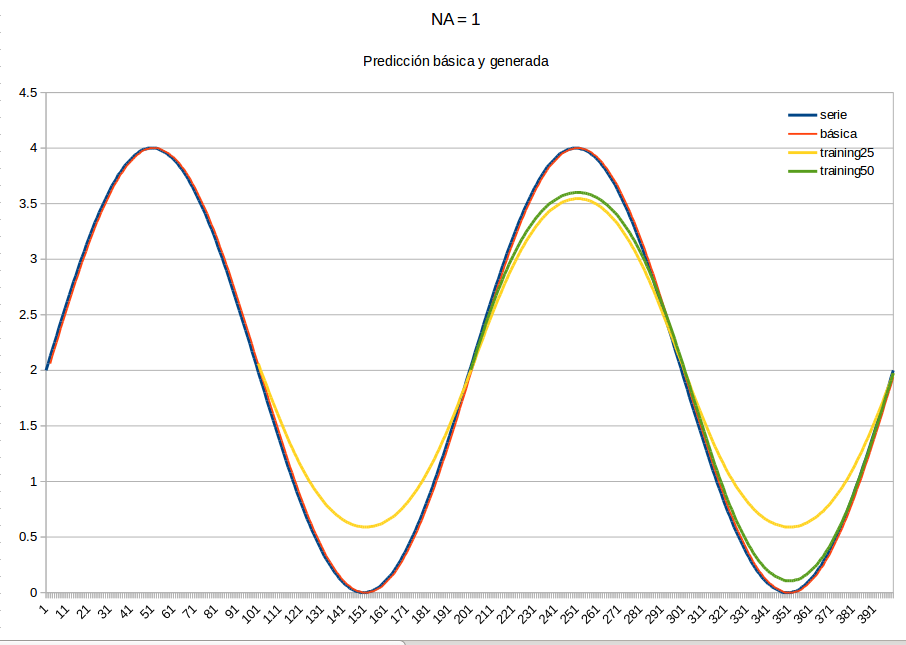
\includegraphics[scale=0.25]{predNA1.png}		
		\caption{Predicciones para NA = 1 y predicción básica (rojo).}				
		\label{pred_no_lineal_ini}
	\end{figure}
	\begin{figure}[H]
		\centering
		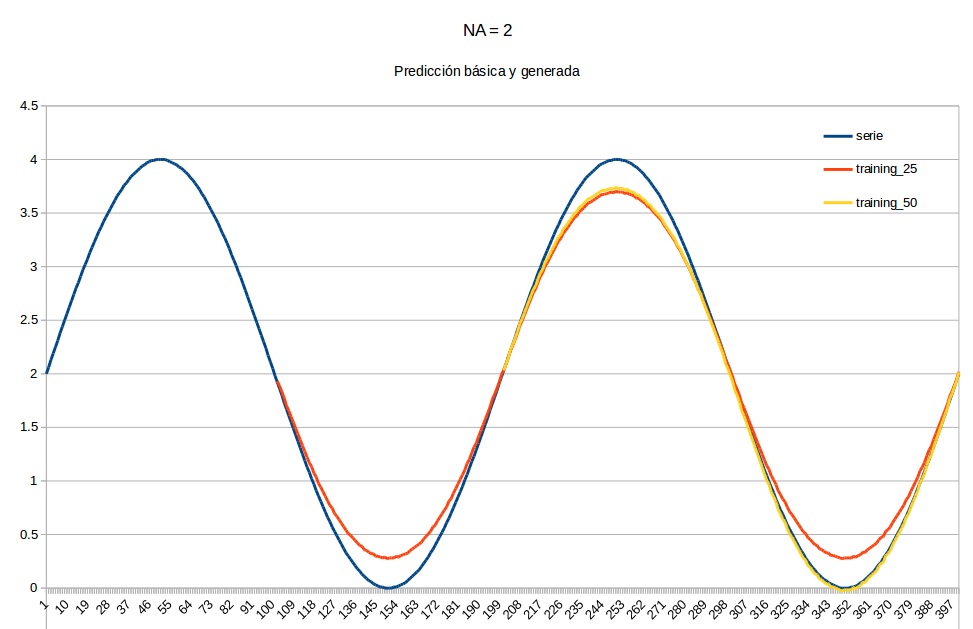
\includegraphics[scale=0.25]{predNA2.png}		
		\caption{Predicciones para NA = 2.}				
	\end{figure}
	\begin{figure}[h]
		\centering
		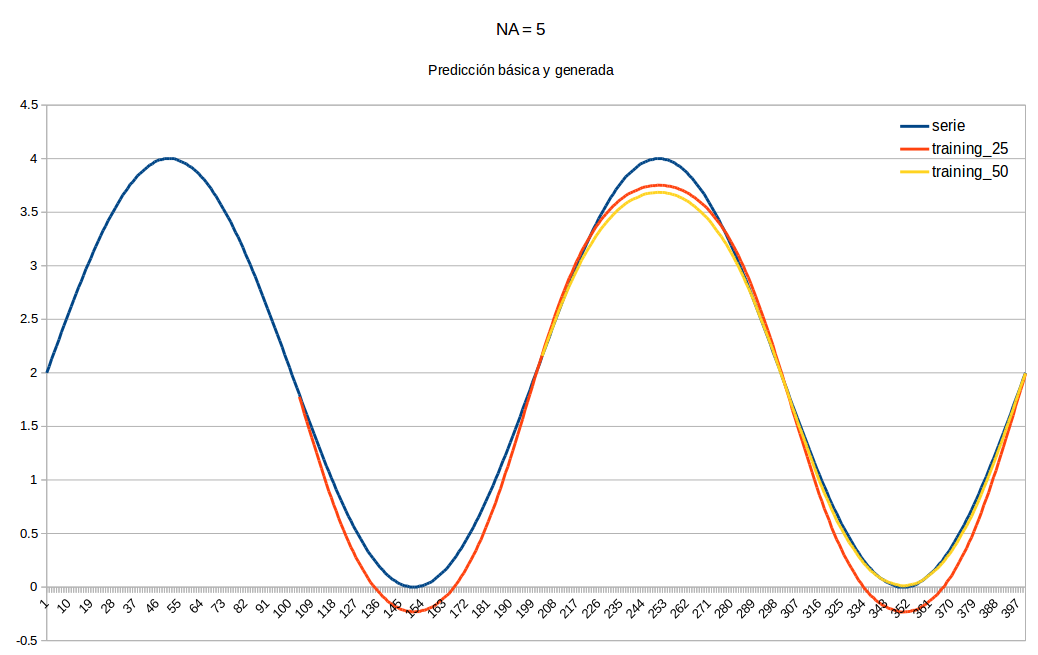
\includegraphics[scale=0.25]{predNA5.png}		
		\caption{Predicciones para NA = 5.}				
		\label{pred_no_lineal_end}
	\end{figure}
	
	Como se puede comprobar en dichas figuras, una de las mejores predicciones en cuanto a similitud de la gráfica es la realizada para NA = 2 y entrenamiento con el 50\% de las muestras (una oscilación completa), no obstante, la predicción realizada para los mismos parámetros, pero con función de transferencia lineal tanto en la capa de salida como en la capa oculta es mucho más precisa y se puede ver en la figura \ref{pred_lineal}.
	
	\begin{figure}[H]
		\centering
		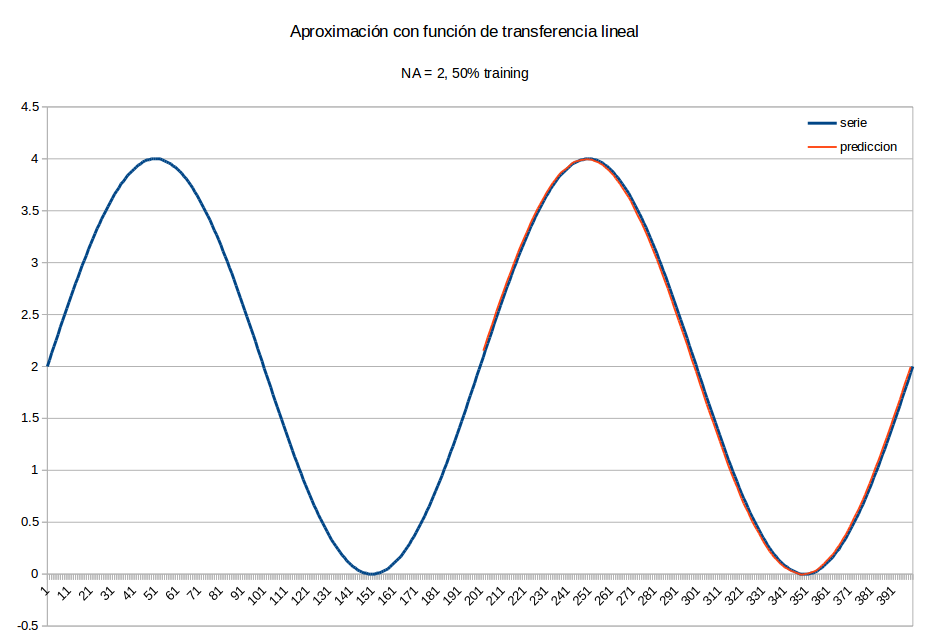
\includegraphics[scale=0.25]{predNA2Lineal.png}		
		\caption{Predicciones para NA = 2 y función de transferencia lineal.}				
		\label{pred_lineal}
	\end{figure}
	
	No obstante se ha detectado una mejora en el error cuadrático medio utilizando la función de transferencia sigmoide cuando se aumenta el número de neuronas en la capa oculta, si bien han sido necesarias 50 neuronas en la capa oculta para bajarlo hasta 0.015744, que sigue siendo mayor que el error de la predicción básica.
	
	\subsection{Ejercicio 9.}
	En la figura \ref{recursive_p1} podemos ver la serie original y la evolución de las predicciones recursivas desde diferentes puntos.
		
	\begin{figure}[H]
		\centering
		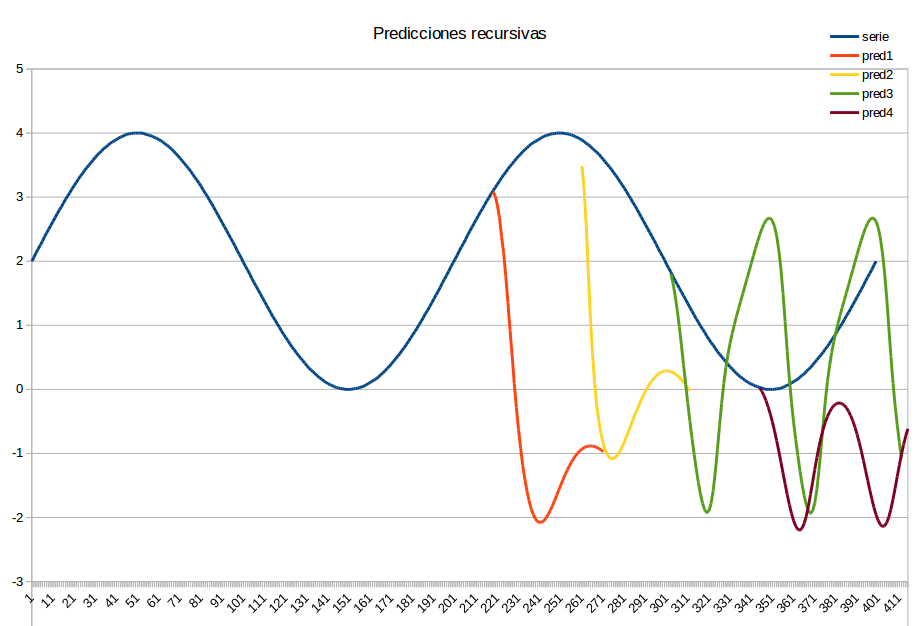
\includegraphics[scale=0.25]{recursive_p1.png}		
		\caption{Predicciones recursivas. NA = 5.}				
		\label{recursive_p1}
	\end{figure}
		
	Como se puede comprobar, la predicción recursiva no es, en absoluto precisa. En ocasiones se ha logrado que la serie que se representa sea bastante similar a una función sinusoidal, pero el período de dicha función suele verse reducido a $\frac{1}{4}$ del período original.
	
	Se ha probado a realizar dichas predicciones con función de transferencia lineal también en la capa oculta obteniendo un resultado que aproxima mejor la función sinusoidal. Se puede ver en la siguiente gráfica.
	
	\begin{figure}[H]
		\centering
		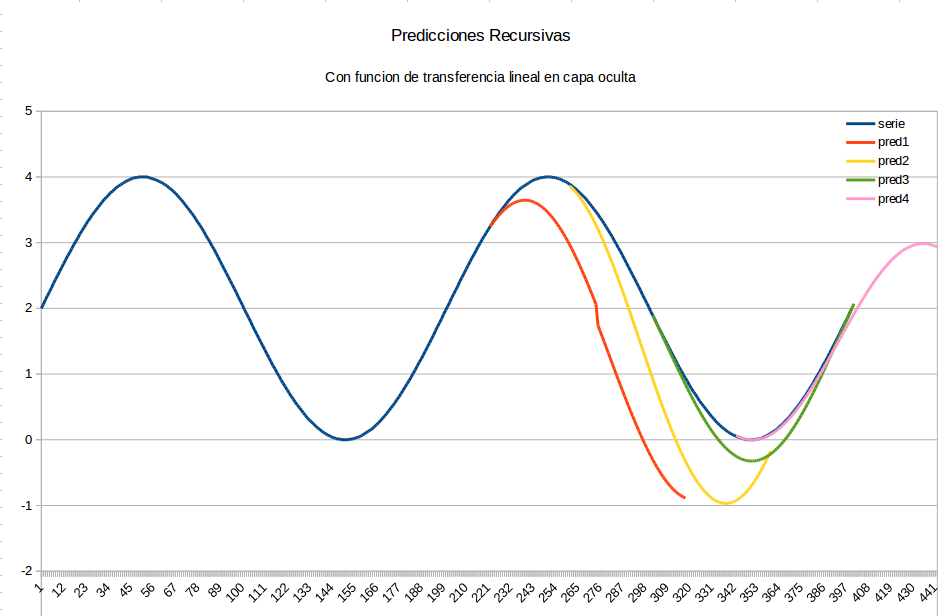
\includegraphics[scale=0.25]{recursive_lin.png}		
		\caption{Predicciones recursivas con transferencia lineal.}				
		\label{recursive_lin}
	\end{figure}
	
	En este caso se puede comprobar como las gráficas se aproximan muy bien inicialmente a la serie temporal original, aunque tras una serie de pasos, el error cometido se acumula y va provocando la separación entre ambas.
	
	\subsection{Ejercicio 10.}
	En la figura \ref{grafico_p2} vemos el aspecto de la serie temporal de la segunda serie proporcionada como material de la práctica y, como se puede ver, esta serie es considerablemente más complicada que la del ejercicio anterior, ya que aparentemente no es periódica.
	
	\begin{figure}[H]
		\centering
		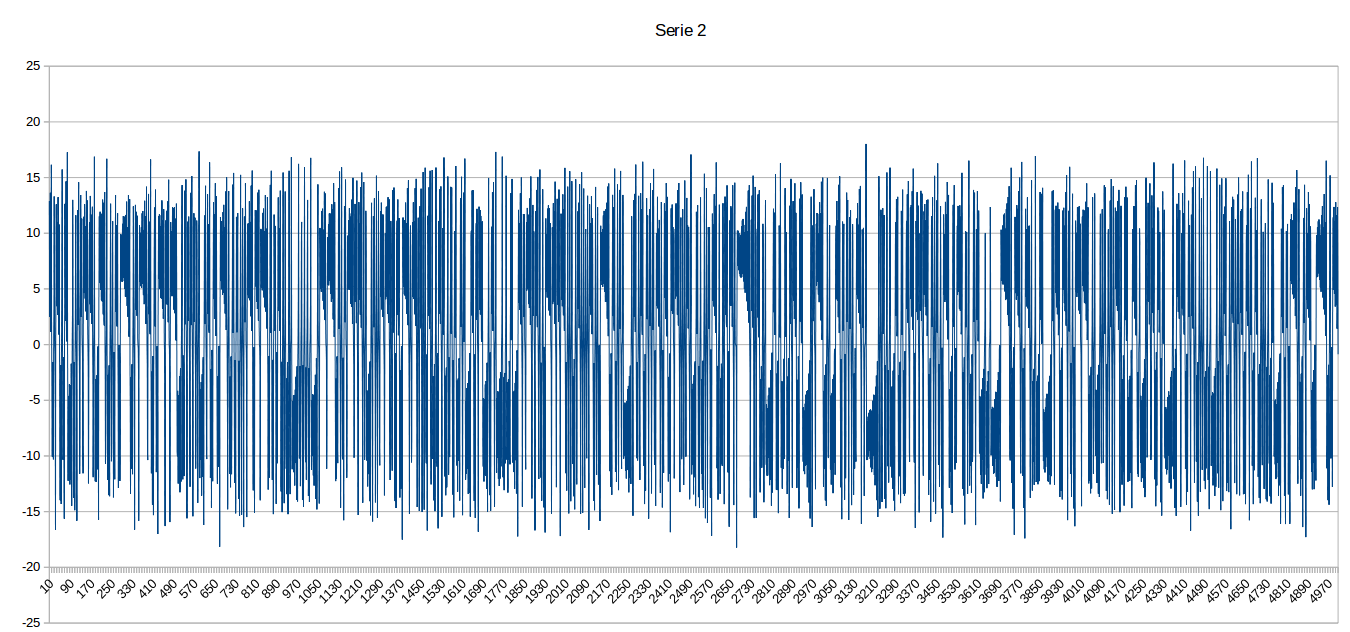
\includegraphics[scale=0.25]{p3_serie2.png}		
		\caption{Serie temporal 2.}				
		\label{grafico_p2}
	\end{figure}
	
	En la siguiente tabla vemos los valores del error cuadrático medio para las diferentes pruebas realizadas, en las que se ha utilizado el 50\% del set de entrenamiento:
	
	\vspace{5mm}
	\noindent\makebox[\textwidth][c]{
		\begin{tabular}{|c|c|c|c|}
			\hline
			& \textbf{NA=1} & \textbf{NA=2} & \textbf{NA=5} \\ \hline
			MSE &    23.855451   &   17.865888     &    11.584109   \\ \hline
			MSE básico &   48.740883   &   48.740883   &   48.748843   \\ \hline
		\end{tabular}
	}
	\vspace{5mm}
	
	Se observa que en esta ocasión aparentemente funciona mejor Na = 5. Para este dato la gráfica con las predicciones es la siguiente:
	
	\begin{figure}[H]
		\centering
		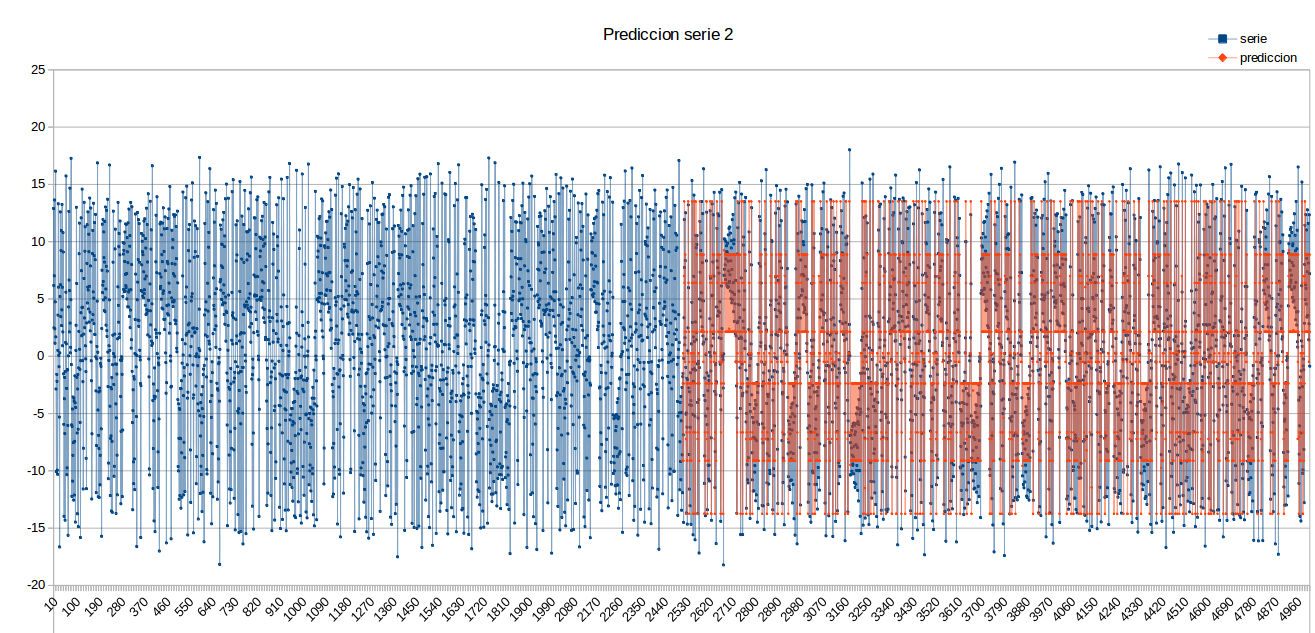
\includegraphics[scale=0.25]{p3_serie2_NA5.png}		
		\caption{Serie temporal y predicciones con NA = 5.}				
		\label{grafico_serie2_predNA5}
	\end{figure}
	
	Podemos observar a simple vista que la predicción se concentra alrededor de unos 10 valores distintos mientras que la serie original no sigue ningún patrón aparente, con lo que la predicción no es buena.
	
	Ante este resultado no podemos esperar una predicción recursiva demasiado precisa, como vemos a continuación.
	
	\begin{figure}[H]
		\centering
		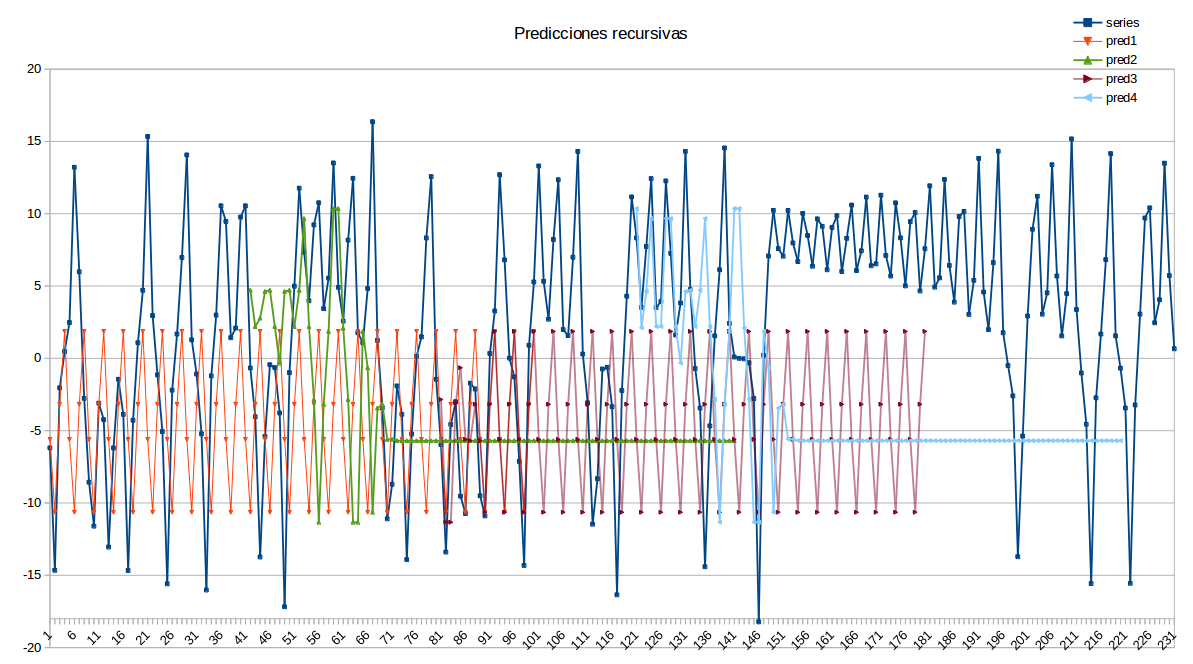
\includegraphics[scale=0.25]{p3_serie2_rec.png}		
		\caption{Serie temporal y predicciones recursivas con NA = 5.}				
		\label{grafico_serie2_predNA5_rec}
	\end{figure}
	
	
	
\end{document}